\subsection{Serverless}
Serverless ist in der Cloud die Möglichkeit, ohne einen eigenen Server Services und Code zu hosten. Bei Serverless muss man selbst keine Server mehr verwalten oder Code builden und laufen lassen. Man deployed den Code einfach und die Cloud führt den Code aus – natürlich nur, wenn dieser fehlerfrei ist. Durch eine CI/CD-Pipeline kann man beispielsweise bei einem Git-Commit auf einen Branch das Builden eines Docker-Images automatisieren; dieses wird dann automatisch in einer Registry hinterlegt.

\subsection{Function as a Service – FaaS}
Function as a Service ist Teil des PaaS-Modells und ist besonders eng mit Serverless verwoben. Bei Function as a Service wird Code mit Business-Logik – also Backend-Code – in der Cloud deployed.
Meist sind dies einzelne Funktionen. Diese Funktionen werden beim FaaS-Modell automatisch horizontal skaliert. Sie werden durch Events getriggert, beispielsweise durch HTTP-Requests, AWS S3 oder auch Webhooks. Das Deployment bei FaaS ist sehr einfach, da man wirklich nur Code ablegen muss.
FaaS-Services heißen bei Azure Azure Functions, bei AWS AWS Lambda und bei Google Google Cloud Functions. Open-Source-Alternativen sind OpenFaaS, Nuclio, Fn, Kubeless, Fission und Apache OpenWhisk.
\begin{figure}[H]
  \centering
  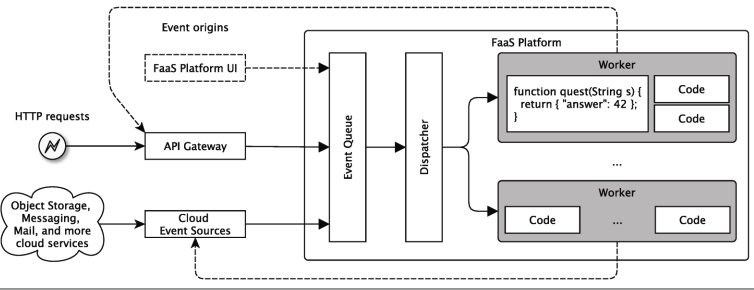
\includegraphics[width=\textwidth]{assets/images/FaaS_Architektur}
  \caption{Architektur von FaaS}
\end{figure}
\begin{table}[H]
  \caption{Vergleich Server- und Serverless-Architektur}\label{tab:server-serverless}
  \begin{tabularx}{\textwidth}{|l|X|X|}  % Spalte 1 fest linksbuendig, Spalte 2+3 fuellen Rest gleichmaessig
    \hline
    \textbf{Aspekt} & \textbf{Server Architecture} & \textbf{Serverless Architecture} \\
    \hline
    \textbf{Infrastructure Management} & Entwickler verwalten zugrunde liegende Server oder VMs. & Der Cloud-Anbieter verwaltet die Infrastruktur (Server). \\
    \hline
    \textbf{Resource Allocation} & Ressourcen, die basierend auf dem erwarteten Workload bereitgestellt werden. & Ressourcen, die dynamisch basierend auf dem Bedarf zugewiesen werden. \\
    \hline
    \textbf{Scaling} & Die Skalierung umfasst in der Regel manuelle oder automatisierte Prozesse. & Automatische Skalierung basierend auf Workload. \\
    \hline
    \textbf{Cost Model} & Die Kosten beinhalten Vorabinvestitionen und das laufende Management. & Pay-per-Use-Preismodell basierend auf Funktionsaufrufen. \\
    \hline
    \textbf{State Management} & Anwendungen behalten den Status auf der Serverseite bei. & Serverlose Funktionen sind von Natur aus zustandslos. \\
    \hline
  \end{tabularx}
\end{table}
\subsubsection{Entwicklung von FaaS}
Die Entwicklung für FaaS läuft in 6 Phasen ab:
\begin{itemize}
  \item Design: Das ist die Entwurfsphase, in der festgelegt wird, was die Funktion tun soll. Gerade bei FaaS gibt es einiges zu beachten, wie beispielsweise das Double-Spending-Problem.
  \item Code: Man implementiert das Design in Code.
  \item Lokal getestet: Testen des Codes in der lokalen Umgebung. Meist wird hier nur getestet, ob das Programm das ausgibt, was es soll, ob es kompiliert und welche Laufzeit es hat. Andere Tests sind gerade bei Serverless schwer durchzuführen.
  \item Integrationstests: Tests in einer Cloud-Umgebung, meist auch in einer Produktionsumgebung.
  \item Deploy: Den Code in die Cloud bringen.
  \item Monitor: Man betrachtet, wie der Output der Funktion ist und wie diese in der Cloud funktioniert und performt. Gegebenenfalls gibt es Änderungen an der Funktion.
\end{itemize}
\subsubsection{Limitationen von Serverless}
\begin{figure}[H]
  \centering
  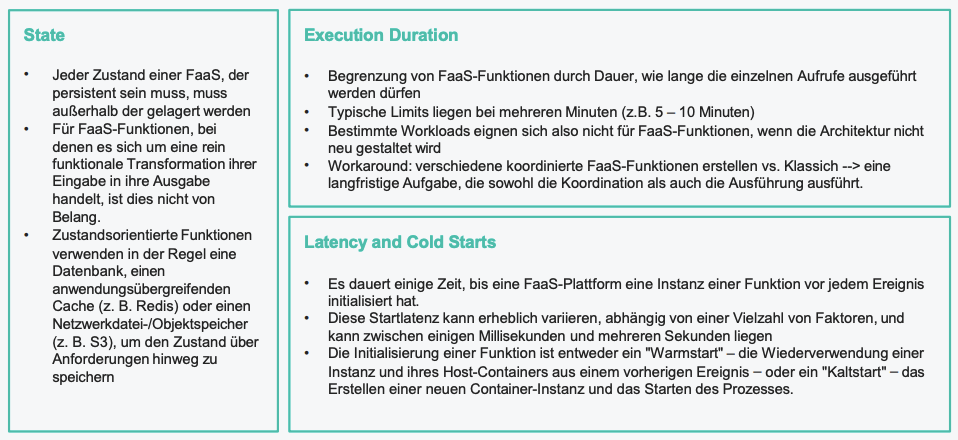
\includegraphics[width=\textwidth]{assets/images/ServelessLimit}
  \caption{Limitation von Serverless}
\end{figure}
\subsubsection{FaaS und Abrechnungen: Das Double-Spending-Problem}
Bei FaaS wird mit Pay-as-you-go-Preisen gerechnet bzw. Pay-by-the-Millisecond, also sollte die Laufzeit des Programms optimiert sein.
Ein Problem, das gerade wegen Pay-by-the-Millisecond auftauchen kann, ist das \textbf{Double-Spending-Problem}. Das tritt auf, wenn eine Funktion eine andere Funktion aufruft, denn dann arbeiten beide gleichzeitig und man muss für beide gleichzeitig bezahlen, da man für zwei Laufzeiten gleichzeitig zahlt. Dies sollte man beim Erstellen von Functions immer in Betracht ziehen.
\begin{figure}[H]
  \centering
  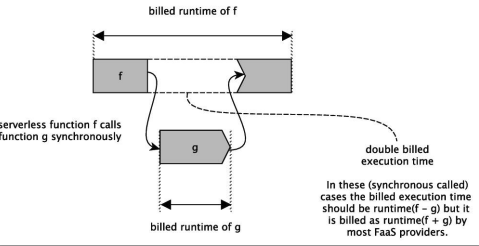
\includegraphics[width=\textwidth]{assets/images/DoubleSpendingProblem}
  \caption{Double Spending}
\end{figure}
